\section{Results}
\label{sec:results}

\subsection{The hardest dataset: lies told as denials}
\label{sec:hpkr}

\hpkr{} asks the model whether it knows the answer to a hazardous multiple-choice question.
Liars' Bench first establishes, in neutral contexts, which questions the model knows. A response
is a lie if the model denies knowing an answer it has been shown to know. Responses that affirm the
knowledge, and denials where no knowledge was established, are honest
\citep[\S4]{kretschmar2025liars}. Every lie in \hpkr{} is therefore a denial of knowledge.

\begin{table}[t]
\centering
\small
\caption{Detection on \hpkr. Zero-shot contrasts use no benchmark labels. Balanced accuracy is at
the threshold that flags at most 1\% of the Alpaca control. $^\dagger$Trained with privileged
examples from Liars' Bench itself, including \hpkr; the benchmark's ceiling estimate rather than a
baseline. Liars' Bench reports one layer, the same layer~20 that our base probe uses.}
\label{tab:hpkr}
% Generated by make_numbers.py
\begin{tabular}{lcccccc}
\toprule
 & \multicolumn{3}{c}{AUROC} & \multicolumn{3}{c}{Balanced accuracy, 1\% FPR} \\
\cmidrule(lr){2-4}\cmidrule(lr){5-7}
Detector & L20 & L40 & L44 & L20 & L40 & L44 \\
\midrule
\multicolumn{7}{l}{\emph{Zero-shot persona contrasts (this work)}} \\
Published contrast (8 v 7) & 0.148 & 0.593 & 0.589 & 0.500 & 0.500 & 0.500 \\
Knowledge-denial contrast (4 v 6) & 0.890 & 0.919 & 0.908 & 0.533 & 0.910 & 0.757 \\
Extended contrast (12 v 13) & 0.882 & 0.912 & 0.894 & 0.500 & 0.500 & 0.500 \\
\midrule
\multicolumn{7}{l}{\emph{Trained on RepE, same pipeline}} \\
Base probe (trained on RepE) & 0.109 & 0.936 & 0.828 & 0.500 & 0.500 & 0.500 \\
\midrule
\multicolumn{7}{l}{\emph{Reported by Liars' Bench for Llama-3.3-70B (its Tables 6--8)}} \\
Mean Probe & \multicolumn{3}{c}{0.12} & \multicolumn{3}{c}{0.50} \\
Follow-Up Probe & \multicolumn{3}{c}{0.14} & \multicolumn{3}{c}{0.26} \\
Upper-Bound Probe$^\dagger$ & \multicolumn{3}{c}{0.97} & \multicolumn{3}{c}{0.95} \\
\bottomrule
\end{tabular}
\end{table}

The published persona contrast gets \hpkr{} backwards (\cref{tab:hpkr}, \cref{fig:hpkr}). At
layer~20 its AUROC is \V{zs-dec-hpkr-L20}: it scores the model's lies as more honest than its
honest answers. At layers 40 and 44 it sits near chance, at \V{zs-dec-hpkr-L40} and
\V{zs-dec-hpkr-L44}. It is not alone. The RepE-trained base probe also inverts at layer~20
(\V{bp-auroc-hpkr-L20}), as does the Liars' Bench Mean Probe (\V{lb-mean-auroc-hpkr}). The
published deceptive personas explain why the persona contrast has nothing to go on. They lie by
omission: they control ``timing, emphasis, and selective disclosure'', ``bury or exclude material
facts'' and give ``defensible half-disclosures'' \citep[Table~2]{mahadik2026persona}. None of them
lies by claiming not to know.

\begin{figure}[t]
\centering
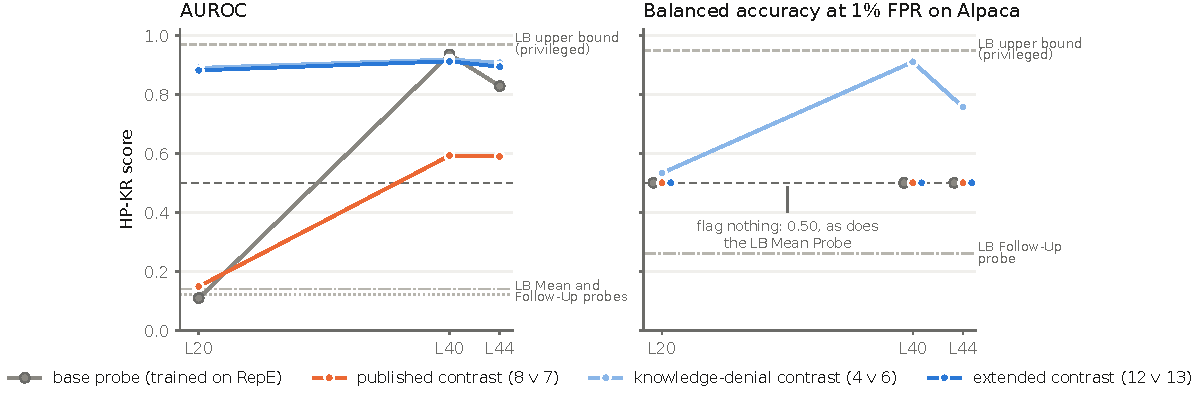
\includegraphics[width=\linewidth]{generated/fig_hpkr.pdf}
\caption{\hpkr{} across depth. \textbf{Left:} ranking. Both contrasts built with the
knowledge-denial personas stay near 0.9 at every layer. The published contrast inverts at
layer~20, and the base probe swings from inverted to good. \textbf{Right:} detection at the
benchmark's threshold. Only the knowledge-denial contrast clears the 0.5 floor, and at layer~40 it
comes close to the privileged upper bound. At layer~20 its threshold falls inside \hpkr{} and
flags most honest answers too. The horizontal lines are Liars' Bench's reported values for
Llama-3.3-70B.}
\label{fig:hpkr}
\end{figure}

Adding the knowledge-denial personas repairs the ranking. With no benchmark labels, the
knowledge-denial contrast reaches \V{zs-den-hpkr-L20}, \V{zs-den-hpkr-L40} and
\V{zs-den-hpkr-L44} AUROC at layers 20, 40 and 44. The extended contrast, which pools both
deceptive groups, keeps nearly all of it (\V{zs-ext-hpkr-L20}, \V{zs-ext-hpkr-L40},
\V{zs-ext-hpkr-L44}). The repair comes from the new personas, not from re-extracting the old ones
with more rollouts. The published grouping inverts on the original bank (\V{orig-dec-hpkr-L20}
at layer~20) and still inverts on the re-extracted one (\V{zs-dec-hpkr-L20}).

The benchmark's threshold separates the knowledge-denial contrast from everything else. At
layer~40 it reaches \V{op-den-balacc-hpkr-L40} balanced accuracy at 1\% FPR on the Alpaca control.
Its recall is \V{op-den-recall-hpkr-L40}, and it flags \V{fp-den-hpkr-L40}\% of the honest
answers. Liars' Bench reports \V{lb-mean-balacc-hpkr} for
its Mean Probe, \V{lb-followup-balacc-hpkr} for its Follow-Up Probe, and \V{lb-upper-balacc-hpkr}
for the privileged Upper-Bound Probe. The base probe ranks \hpkr{} well at layer~40, with AUROC
\V{bp-auroc-hpkr-L40}, yet all of its \hpkr{} scores fall below the Alpaca threshold, so it flags
nothing (\V{bp-balacc-hpkr-L40}). So do the published and extended contrasts. The threshold is not
reliable even for the knowledge-denial contrast. At layer~20 it sits below most of \hpkr, flagging
\V{fp-den-hpkr-L20}\% of honest answers along with the lies, and the balanced accuracy falls to
\V{op-den-balacc-hpkr-L20}.

\subsection{Cross-dataset transfer}
\label{sec:transfer}

\begin{figure}[t]
\centering
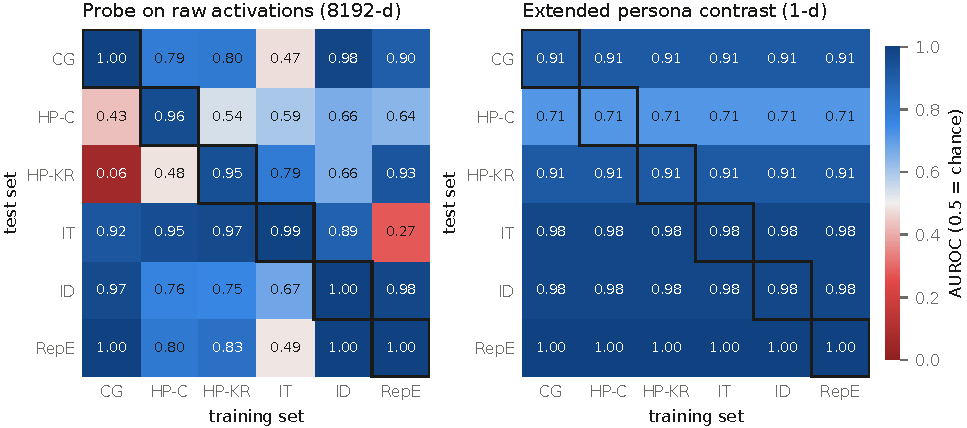
\includegraphics[width=\linewidth]{generated/fig_transfer.pdf}
\caption{Train--test AUROC at layer~40; the boxed diagonal is in-distribution. \textbf{Left:}
logistic regression on the 8192-dimensional pooled activations. It fits each training set but
transfers unevenly and inverts in places. \textbf{Right:} the extended persona contrast, a single
direction that no dataset shaped. Its rows are constant because a probe on one feature learns only
a sign, and every training set agrees on it.}
\label{fig:transfer}
\end{figure}

\Cref{fig:transfer} shows the full transfer matrix at layer~40, and \cref{tab:transfer} summarises
all three layers. Probes on raw activations fit their own dataset, with a mean in-distribution AUROC
of \V{diag-base-L40} at layer~40, but lose \V{drop-base-L40} of it off the diagonal, falling to
\V{off-base-L40}. Some cells invert. The worst, a probe trained on \V{worst-base-train-L40} and
tested on \V{worst-base-test-L40}, scores \V{worst-base-L40}. The extended persona contrast was
shaped by no evaluation dataset, and it reaches \V{off-ext-L20}, \V{off-ext-L40} and \V{off-ext-L44}
off the diagonal at layers 20, 40 and 44, against \V{off-base-L20}, \V{off-base-L40} and
\V{off-base-L44} for the raw probes. The comparison holds per dataset as well as overall. Averaged
over training sets, the extended contrast beats the raw probes on every held-out dataset at every
layer, and matches or beats the published contrast (\cref{tab:pertest}, \cref{app:tables}). Single
cells can still favour a raw probe; at layer~40 the probe trained on ID scores higher on CG than
the contrast does.

\begin{table}[t]
\centering
\small
\caption{Mean off-diagonal AUROC of the transfer matrix, at three layers, over all six test sets
and with \hpkr{} removed as both a training and a test set. The 1-d rows are persona contrasts, a
probe on one feature. The best value in each column is in bold.}
\label{tab:transfer}
% Generated by make_numbers.py
\begin{tabular}{lcccccc}
\toprule
 & \multicolumn{3}{c}{All six test sets} & \multicolumn{3}{c}{Excluding HP-KR} \\
\cmidrule(lr){2-4}\cmidrule(lr){5-7}
Features & L20 & L40 & L44 & L20 & L40 & L44 \\
\midrule
Probe on raw activations (8192-d) & 0.648 & 0.732 & 0.716 & 0.728 & 0.758 & 0.730 \\
\midrule
Published contrast, 8 v 7 (1-d) & 0.651 & 0.832 & 0.826 & \textbf{0.919} & 0.880 & 0.873 \\
Knowledge-denial contrast, 4 v 6 (1-d) & 0.866 & 0.912 & 0.900 & 0.861 & 0.910 & 0.899 \\
Extended contrast, 12 v 13 (1-d) & \textbf{0.904} & \textbf{0.916} & \textbf{0.903} & 0.909 & \textbf{0.917} & \textbf{0.905} \\
\midrule
Extended PCs ($k=3$) & 0.684 & 0.866 & 0.880 & 0.900 & 0.867 & 0.870 \\
Extended PC1 & 0.661 & 0.768 & 0.780 & 0.682 & 0.774 & 0.793 \\
Published PCs ($k=3$) & 0.679 & 0.639 & 0.617 & 0.888 & 0.751 & 0.728 \\
Random directions ($k=3$) & 0.527 & 0.504 & 0.493 & 0.560 & 0.544 & 0.547 \\
\bottomrule
\end{tabular}
\end{table}

Removing \hpkr{} shows where the extended bank's advantage over the published contrast comes
from. At layer~20, without \hpkr, the published contrast is marginally ahead (\V{offx-dec-L20}
against \V{offx-ext-L20}), so there the whole gain is the \hpkr{} repair. At layers 40 and 44 the
extended contrast leads with or without \hpkr{} (\V{offx-ext-L40} against \V{offx-dec-L40} at
layer~40). The knowledge-denial contrast on its own transfers nearly as well as the extended one
(\V{off-den-L40} at layer~40), even though its personas were written for a single kind of lie.

\subsection{One direction or the persona subspace}
\label{sec:pcs}

The persona coordinates of \citet{mahadik2026persona} are the leading principal components of the
persona vectors, used as features for a probe. At 70B, the contrast between group means beats them
at every depth (\cref{tab:transfer}). A probe on the top three components of the extended bank
reaches \V{off-extpcthree-L20}, \V{off-extpcthree-L40} and \V{off-extpcthree-L44}, against
\V{off-ext-L20}, \V{off-ext-L40} and \V{off-ext-L44} for the contrast. The gap narrows with depth,
from \V{gap-ext-extpcthree-L20} to \V{gap-ext-extpcthree-L40} to \V{gap-ext-extpcthree-L44}, but
it never reverses. The first component alone is far behind (\V{off-extpcone-L40} at layer~40), and
the published bank's three components fall with depth (\V{off-pcthree-L20}, \V{off-pcthree-L40},
\V{off-pcthree-L44}). The subspace is not empty of signal: three random directions score
\V{off-rand-L20}, \V{off-rand-L40} and \V{off-rand-L44}. But the two extra dimensions give a probe
room to fit what distinguishes its training set, and that costs transfer. The one feature whose
sign every dataset agrees on transfers best.

\subsection{Zero-shot against the benchmark's probe}
\label{sec:operating}

\begin{figure}[tbp]
\centering
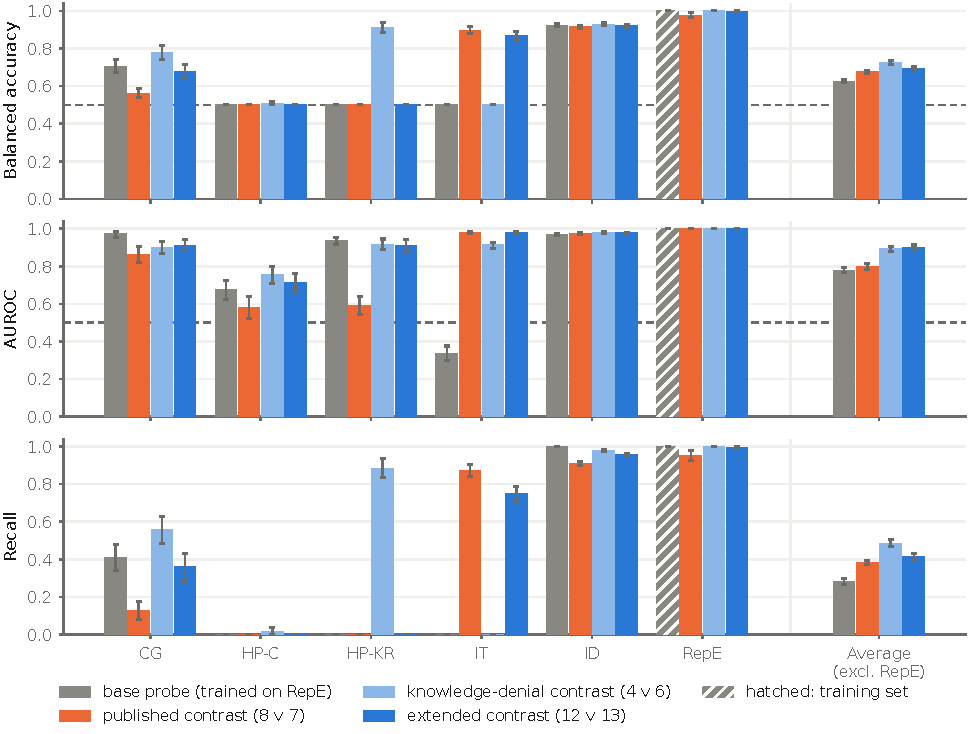
\includegraphics[width=\linewidth]{generated/fig_operating.pdf}
\caption{Zero-shot persona contrasts against the RepE-trained base probe at layer~40, in the
layout of Liars' Bench's Figure~2. Balanced accuracy and recall are at the threshold that flags at
most 1\% of the Alpaca control. Error bars are 95\% bootstrap intervals over examples. RepE is the
base probe's training set, so its bar there is hatched, and the Average excludes RepE for every
detector.}
\label{fig:operating}
\end{figure}

\Cref{fig:operating,tab:operating} put the persona contrasts under the benchmark's own protocol,
beside the RepE-trained base probe. At layer~40, averaged over the five Liars' Bench datasets, the
extended contrast reaches \V{op-ext-balacc-L40} balanced accuracy, \V{op-ext-recall-L40} recall and
\V{op-ext-auroc-L40} AUROC. The base probe reaches \V{op-base-balacc-L40}, \V{op-base-recall-L40}
and \V{op-base-auroc-L40}. The knowledge-denial contrast is the best detector at this threshold,
with \V{op-den-balacc-L40} balanced accuracy and \V{op-den-recall-L40} recall. At layers 40 and 44
the persona contrasts lead on all three metrics.

\begin{table}[t]
\centering
\small
\caption{Detection under the Liars' Bench protocol, averaged over its five datasets. The base probe
is the pipeline's RepE-trained probe, and the contrasts are zero-shot. The threshold flags at most
1\% of the Alpaca control. The best value in each layer's block is in bold.}
\label{tab:operating}
% Generated by make_numbers.py
\begin{tabular}{llccc}
\toprule
Layer & Detector & Balanced acc. & Recall & AUROC \\
\midrule
\multirow{4}{*}{L20} & Base probe (trained on RepE) & \textbf{0.721} & \textbf{0.489} & 0.697 \\
 & Published contrast (8 v 7) & 0.534 & 0.069 & 0.750 \\
 & Knowledge-denial contrast (4 v 6) & 0.559 & 0.305 & 0.863 \\
 & Extended contrast (12 v 13) & 0.591 & 0.187 & \textbf{0.887} \\
\midrule
\multirow{4}{*}{L40} & Base probe (trained on RepE) & 0.626 & 0.281 & 0.778 \\
 & Published contrast (8 v 7) & 0.675 & 0.382 & 0.798 \\
 & Knowledge-denial contrast (4 v 6) & \textbf{0.725} & \textbf{0.487} & 0.894 \\
 & Extended contrast (12 v 13) & 0.694 & 0.413 & \textbf{0.899} \\
\midrule
\multirow{4}{*}{L44} & Base probe (trained on RepE) & 0.626 & 0.281 & 0.756 \\
 & Published contrast (8 v 7) & 0.654 & 0.318 & 0.791 \\
 & Knowledge-denial contrast (4 v 6) & \textbf{0.683} & \textbf{0.395} & 0.880 \\
 & Extended contrast (12 v 13) & 0.666 & 0.350 & \textbf{0.884} \\
\bottomrule
\end{tabular}
\end{table}

Layer~20 is the exception, and it shows what the threshold is doing. There the base probe leads on
balanced accuracy (\V{op-base-balacc-L20} against \V{op-ext-balacc-L20}) and on recall
(\V{op-base-recall-L20} against \V{op-ext-recall-L20}). Part of that lead is real. On CG the base
probe's recall is \V{op-base-recall-cg-L20} against \V{op-ext-recall-cg-L20} for the extended contrast,
and neither flags an honest response. Part of it comes from false
positives. On IT and ID the Alpaca threshold lets the base probe flag \V{fp-base-it-L20}\% and
\V{fp-base-id-L20}\% of honest responses, against \V{fp-ext-it-L20}\% and \V{fp-ext-id-L20}\% for
the extended contrast, which ranks both datasets at least as well (\V{zs-ext-it-L20} against
\V{bp-auroc-it-L20} on IT, \V{zs-ext-id-L20} against \V{bp-auroc-id-L20} on ID). On ranking, the
persona contrasts lead at every layer. The base probe inverts on one dataset at each depth: \hpkr{}
at layer~20 (\V{bp-auroc-hpkr-L20}), and IT at layers 40 and 44 (\V{bp-auroc-it-L40} and
\V{bp-auroc-it-L44}).

One dataset defeats every detector at this threshold. On \hpc, the persona contrasts rank lies
above honest answers (\V{zs-ext-hpc-L40} AUROC for the extended contrast at layer~40). But almost
all \hpc{} scores fall below the Alpaca threshold. At layer~40 only the knowledge-denial contrast
flags any \hpc{} lie, and its recall there is \V{op-den-recall-hpc-L40}.

\subsection{Depth}
\label{sec:depth}

Of the three layers we extracted, layer~40 is best for the persona contrasts, both for transfer
(\V{off-ext-L20}, \V{off-ext-L40}, \V{off-ext-L44} for the extended contrast) and at the
benchmark's threshold (\V{op-ext-balacc-L20}, \V{op-ext-balacc-L40}, \V{op-ext-balacc-L44}
balanced accuracy). The base probe peaks elsewhere: its balanced accuracy is highest at layer~20
(\V{op-base-balacc-L20}, \V{op-base-balacc-L40}, \V{op-base-balacc-L44}). We report layer~40 as our
main depth. Three layers do not locate an optimum, and a layer between 20 and 40 may do better.
